%With the advent of multicore processors, research into multi-threading is gaining popularity. Researchers are looking into development of algorithms which can execute efficiently on multicore systems.\\ 
With the advent of multicore processors, development of performance tools and algorithms targeted for parallel architectures has been given a boost. Many research areas  provide a wide variety of problems whose would show improved performance when executed in parallel. One such area is scientific and numerical computing. Scientic algorithms are used by researchers from a variety of fields such as chemistry, biology, geography etc. as well as different sub-fields of computer science like machine learning. In most cases, these algorithms are written in languages  that are collectively known as  array based languages. A few examples of such languages are  \matlab, R and Python with it's NumPy library.\\
Array based languages offer a variety of features including a interpreter style read-eval-print-eval,functions such as eval and feval for dynamic code evaluation,  no types etc. which enable rapid prototyping. However due to the very same features, these languages show poorer performance when compared to statically compiled languages. A common approach for improving the performance is compile whole programs to languages such as {\sc FORTRAN} and C. However, in most cases, the most computationally intensive portion of the program is small, often localised inside a loop body. Hence compiling the entire program is not necessary. In most cases speed up observed through partial compilation of hot code sections is commensurate with that observed by compiling the whole program. This allows the user to continue programming in the language he/she is more comfortable in.\\
Array based languages such as \matlab \cite{matlab} and Python, with it's NumPy library are popular among scientists and mathematicians for writing   numerical and scientific programs. These languages offer a variety of features including a interpreter style read-eval-print-eval, no types etc which enable rapid prototyping. However due to the very same features, these languages show poorer performance when compared to statically compiled languages. A common approach for improving the performance is compile whole programs to languages such as {\sc FORTRAN} and C. However, in most cases, the most computationally intensive portion of the program is small, often localised inside a loop body. Hence compiling the entire program is not necessary. In most cases speed up observed through partial compilation of hot code sections is commensurate with that observed by compiling the whole program. This allows the user to continue programming in the language he/she is more comfortable in.\\

This thesis addresses the problem of improving the performance of programs written in array based languages by compiling the hot sections to parallel C++. We support both \matlab and Numpy. There are two main challenges. First one is supporting the different and often complementary semantics of both languages. The other is supporting the large number of builtins methods that are supported by both languages.
Our solution implement a static C++ backend for velociraptor toolkit and use tools to compile matlab and python programs to the velociraptor intermediate representation. The McLab static pipeline is used for \matlab and PyVrir, a proof of concept Python frontend for Velociraptor is used for Python. 

\begin{figure}[htbp]
\begin{center}
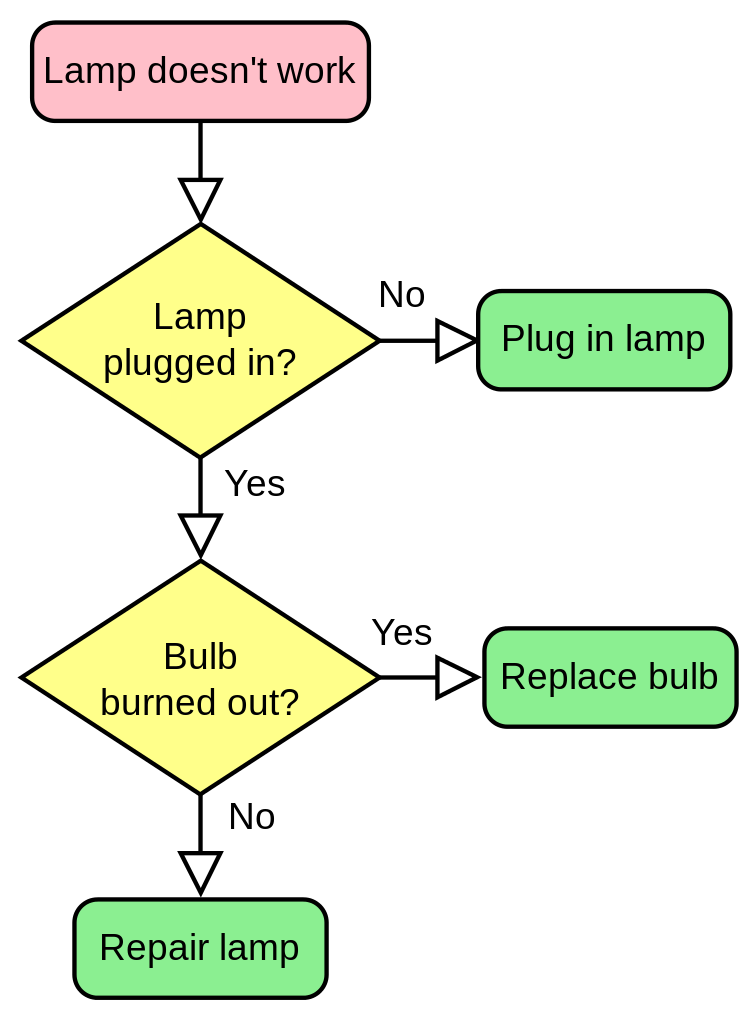
\includegraphics[width=3.5in]{Figures/overview.png}
\caption[Overview of the \matlab Tamer]{Overview
of our \matlab Tamer.  The shaded boxes indicate the components
presented in this thesis.  The other solid boxes correspond to
existing \mclab tools we use, and the dashed boxes correspond to
ongoing projects which are using the results of this
thesis.}\label{Fig:Overview}
\end{center}
\end{figure}
\section{Contributions}
The main contributions of this thesis are as follows.
\begin{itemize}
\item Generating the velociraptor intermediate representation from the McSAF intermediate representation. 
\item Converting Colon expressions to Range expressions
\item Generating glue code necessary for invoking C++ functions from \matlab.
\item Generating C++ code from the velociraptor IR.
\item Optmising generated code by elminating bounds checks unncessary memory allocations. 
\end{itemize}
\section{Thesis Outline}
This thesis is divided into \ref{chap:Conclusions} chapters, including this one, which are structured as follows.
\chapref{chap: Background} gives a brief overview of the tools
used by VeloCty.
\chapref{chap: McSAFTranslate} describes the translation from the McSAF  
intermediate representation to the Velociraptor intermediate representation(VRIR).
\chapref{chap: glueCode} describes the various aspects of generating glue code for \matlab's Mex API including how input data is converted from Mex data structures to VeloCty data structures. 
\chapref{chap: vrirBackend} talks about the generation of C++ code from VRIR.
\chapref{chap: codeOptimise} explains the code optimisations implemented to improve the performance. 
\chapref{chap:Related} provides an overview of related work and
\chapref{chap:Conclusions} concludes.
